\documentclass[11pt,letterpaper]{article}
\usepackage{../assets/scientific_report}
\usepackage{pgfplots}
\pgfplotsset{compat=1.18}
\usepackage{float}
\usepackage{listings}
\usepackage{xcolor}
\usepackage{geometry}
\geometry{headheight=23pt, top=2cm, bottom=2cm, left=2.5cm, right=2.5cm}
\setlength{\parskip}{0.5em}
\setlength{\parindent}{0pt}

\lstset{
    language=C,
    basicstyle=\ttfamily\small,
    keywordstyle=\color{blue}\bfseries,
    commentstyle=\color{green!60!black}\itshape,
    stringstyle=\color{red!80!black},
    numbers=left,
    numberstyle=\tiny\color{gray},
    numbersep=8pt,
    frame=single,
    breaklines=true,
    captionpos=b,
    tabsize=4,
    showstringspaces=false
}

\begin{document}
\pagestyle{plain}

\begin{center}
    {\LARGE\bfseries Multiplicação de Matriz por Vetor (MxV):}\\[0.3em]
    {\LARGE\bfseries Acesso por Linhas vs Acesso por Colunas}\\[0.5em]
    {\large Análise de Desempenho e Padrões de Acesso à Memória}\\[1em]
    {\normalsize Eugênio Vitor Lopes dos Santos}\\[0.3em]
    {\small DCA3703 -- Programação Paralela, Universidade Federal do Rio Grande do Norte}\\[0.3em]
    {\small 2026}
\end{center}

\vspace{1em}

\section{Enunciado}

Implemente duas versões da multiplicação de matriz por vetor (MxV) em C: uma com acesso à matriz por linhas (laço interno variando coluna) e outra por colunas (laço interno variando linha). Meça o tempo de execução de cada versão com uma função apropriada e execute testes com diferentes tamanhos de matriz. Identifique a partir de que tamanho os tempos passam a divergir significativamente e explique por que isso ocorre, relacionando suas observações com o uso da memória cache e o padrão de acesso à memória.

\section{Fundamentação Teórica}

\subsection{Multiplicação de Matriz por Vetor (MxV)}

A operação MxV calcula $y = A \cdot x$, onde $A$ é uma matriz $N \times N$ e $x$ é um vetor de tamanho $N$:
\[
y_i = \sum_{j=0}^{N-1} A[i][j] \cdot x[j], \quad i = 0, 1, \ldots, N-1
\]

\subsection{Ordem dos Laços e Disposição em Memória}

Em C, matrizes bidimensionais são organizadas em ordem por linhas (\textit{row-major order}). Elementos consecutivos da mesma linha ocupam posições contíguas na memória. A ordem de iteração nos laços determina diretamente se o acesso aproveita essa contiguidade física.

No acesso por linhas, o laço externo percorre $i$ e o interno percorre $j$. A expressão $A[i \cdot N + j]$ visita $A[0][0], A[0][1], A[0][2], \ldots$ com passo unitário de 8 bytes (para o tipo \texttt{double}). Já no acesso por colunas, o laço externo percorre $j$ e o interno percorre $i$. Cada iteração do laço interno avança $N$ elementos na memória ($8N$ bytes), saltando linhas inteiras a cada operação.

\subsection{Hierarquia de Cache e Localidade de Referência}

A hierarquia de memória baseia-se em dois princípios fundamentais:
\begin{itemize}
    \item \textbf{Localidade temporal.} Dados acessados recentemente permanecem no cache para acelerar acessos futuros imediatos.
    \item \textbf{Localidade espacial.} Ao buscar uma palavra da memória, o processador transfere um bloco contíguo inteiro (\textit{cache line} de 64 bytes), antecipando acessos a endereços adjacentes.
\end{itemize}

O processador utilizado nos testes é um Intel Core i7-14700HX (20 núcleos físicos, 28 threads lógicas). A Tabela~\ref{tab:cache} descreve a topologia de cache da máquina.

\begin{table}[H]
\centering
\caption{Hierarquia de cache da máquina de teste (Intel Core i7-14700HX).}
\label{tab:cache}
\small
\begin{tabular}{@{}llr@{}}
\toprule
\textbf{Nível} & \textbf{Tipo} & \textbf{Capacidade} \\
\midrule
L1D & Dados, privativo por núcleo & 48 KiB \\
L1I & Instruções, privativo por núcleo & 32 KiB \\
L2  & Unificado, privativo por núcleo & 2 MiB \\
L3  & Unificado, compartilhado & 33 MiB \\
\bottomrule
\end{tabular}
\end{table}

\subsection{Linha de Cache e Transferência de Dados}

A unidade atômica de transferência entre a memória principal e os níveis de cache é a linha de cache (\textit{cache line}), de 64 bytes. Cada linha comporta exatamente 8 valores de tipo \texttt{double} (8 bytes cada). 

No acesso por linhas, a primeira leitura traz 64 bytes contíguos da memória; os 7 acessos seguintes consomem os dados que já estão no cache L1, sem penalidade de latência adicional. No acesso por colunas com $N \ge 8$, cada leitura sucessiva busca um endereço deslocado por $8N$ bytes, caindo em uma linha de cache diferente. O processador carrega 64 bytes para utilizar apenas 8, desperdiçando 87,5\% da largura de banda transferida.

\newpage
\section{Experimento}

\subsection{Código-Fonte}

\begin{lstlisting}[caption={Acesso por linhas (row-major)}, label={lst:row}]
#define _POSIX_C_SOURCE 199309L
#include <stdio.h>
#include <stdlib.h>
#include <time.h>

static double agora(void) {
    struct timespec t;
    clock_gettime(CLOCK_MONOTONIC, &t);
    return t.tv_sec + t.tv_nsec / 1e9;
}

int main(int argc, char *argv[]) {
    int N = 2000;
    if (argc > 1) N = atoi(argv[1]);

    double *A = malloc((size_t)N * N * sizeof(double));
    double *x = malloc(N * sizeof(double));
    double *y = calloc(N, sizeof(double));

    for (int i = 0; i < N * N; i++) A[i] = 1.0;
    for (int i = 0; i < N; i++) x[i] = 1.0;

    double inicio = agora();

    for (int i = 0; i < N; i++) {
        double s = 0.0;
        for (int j = 0; j < N; j++)
            s += A[i * N + j] * x[j];
        y[i] = s;
    }

    double fim = agora();
    double tempo = fim - inicio;
    printf("Row-major  N=%d  tempo=%.6f s  y[0]=%.1f\n",
           N, tempo, y[0]);

    free(A); free(x); free(y);
    return 0;
}
\end{lstlisting}

\newpage
\begin{lstlisting}[caption={Acesso por colunas (column-major)}, label={lst:col}]
#define _POSIX_C_SOURCE 199309L
#include <stdio.h>
#include <stdlib.h>
#include <time.h>

static double agora(void) {
    struct timespec t;
    clock_gettime(CLOCK_MONOTONIC, &t);
    return t.tv_sec + t.tv_nsec / 1e9;
}

int main(int argc, char *argv[]) {
    int N = 2000;
    if (argc > 1) N = atoi(argv[1]);

    double *A = malloc((size_t)N * N * sizeof(double));
    double *x = malloc(N * sizeof(double));
    double *y = calloc(N, sizeof(double));

    for (int i = 0; i < N * N; i++) A[i] = 1.0;
    for (int i = 0; i < N; i++) x[i] = 1.0;

    double inicio = agora();

    for (int j = 0; j < N; j++) {
        for (int i = 0; i < N; i++)
            y[i] += A[i * N + j] * x[j];
    }

    double fim = agora();
    double tempo = fim - inicio;
    printf("Column-major  N=%d  tempo=%.6f s  y[0]=%.1f\n",
           N, tempo, y[0]);

    free(A); free(x); free(y);
    return 0;
}
\end{lstlisting}

\newpage
Os vetores e matrizes foram alocados e preenchidos antes de iniciar o cronômetro, isolando exclusivamente o laço de cálculo da multiplicação. O código foi compilado com GCC sem otimizações (\texttt{-O0}) para impedir que o compilador reordenasse os laços ou vetorizasse os acessos automaticamente:

\begin{lstlisting}[caption={Compilação e execução dos testes}, label={lst:exec}]
gcc row_major.c -o row_major -O0
gcc column_major.c -o column_major -O0
./row_major 2000
./column_major 2000
\end{lstlisting}

\section{Resultados}

\begin{table}[H]
\centering
\caption{Tempos de execução medidos para a multiplicação matriz-vetor.}
\label{tab:results}
\small
\begin{tabular}{@{}lcc@{}}
\toprule
\textbf{N} & \textbf{Row-major (s)} & \textbf{Column-major (s)} \\
\midrule
10    & 0.002295 & 0.002831 \\
20    & 0.001866 & 0.001827 \\
30    & 0.001956 & 0.002252 \\
40    & 0.002174 & 0.002068 \\
50    & 0.002315 & 0.002776 \\
100   & 0.001963 & 0.002202 \\
200   & 0.002168 & 0.002965 \\
300   & 0.002709 & 0.003243 \\
400   & 0.003879 & 0.004282 \\
500   & 0.005708 & 0.004723 \\
600   & 0.005673 & 0.005695 \\
700   & 0.006593 & 0.008838 \\
800   & 0.008769 & 0.007560 \\
900   & 0.010388 & 0.009706 \\
1000  & 0.009775 & 0.011743 \\
1200  & 0.013580 & 0.015531 \\
1400  & 0.017189 & 0.018966 \\
1600  & 0.019798 & 0.023868 \\
1800  & 0.027032 & 0.034185 \\
2000  & 0.031170 & 0.039495 \\
2500  & 0.044809 & 0.069988 \\
3000  & 0.071794 & 0.092323 \\
3500  & 0.087319 & 0.140740 \\
4000  & 0.115090 & 0.200937 \\
4500  & 0.141870 & 0.239610 \\
5000  & 0.154810 & 0.252379 \\
\bottomrule
\end{tabular}
\end{table}

\begin{figure}[H]
\centering
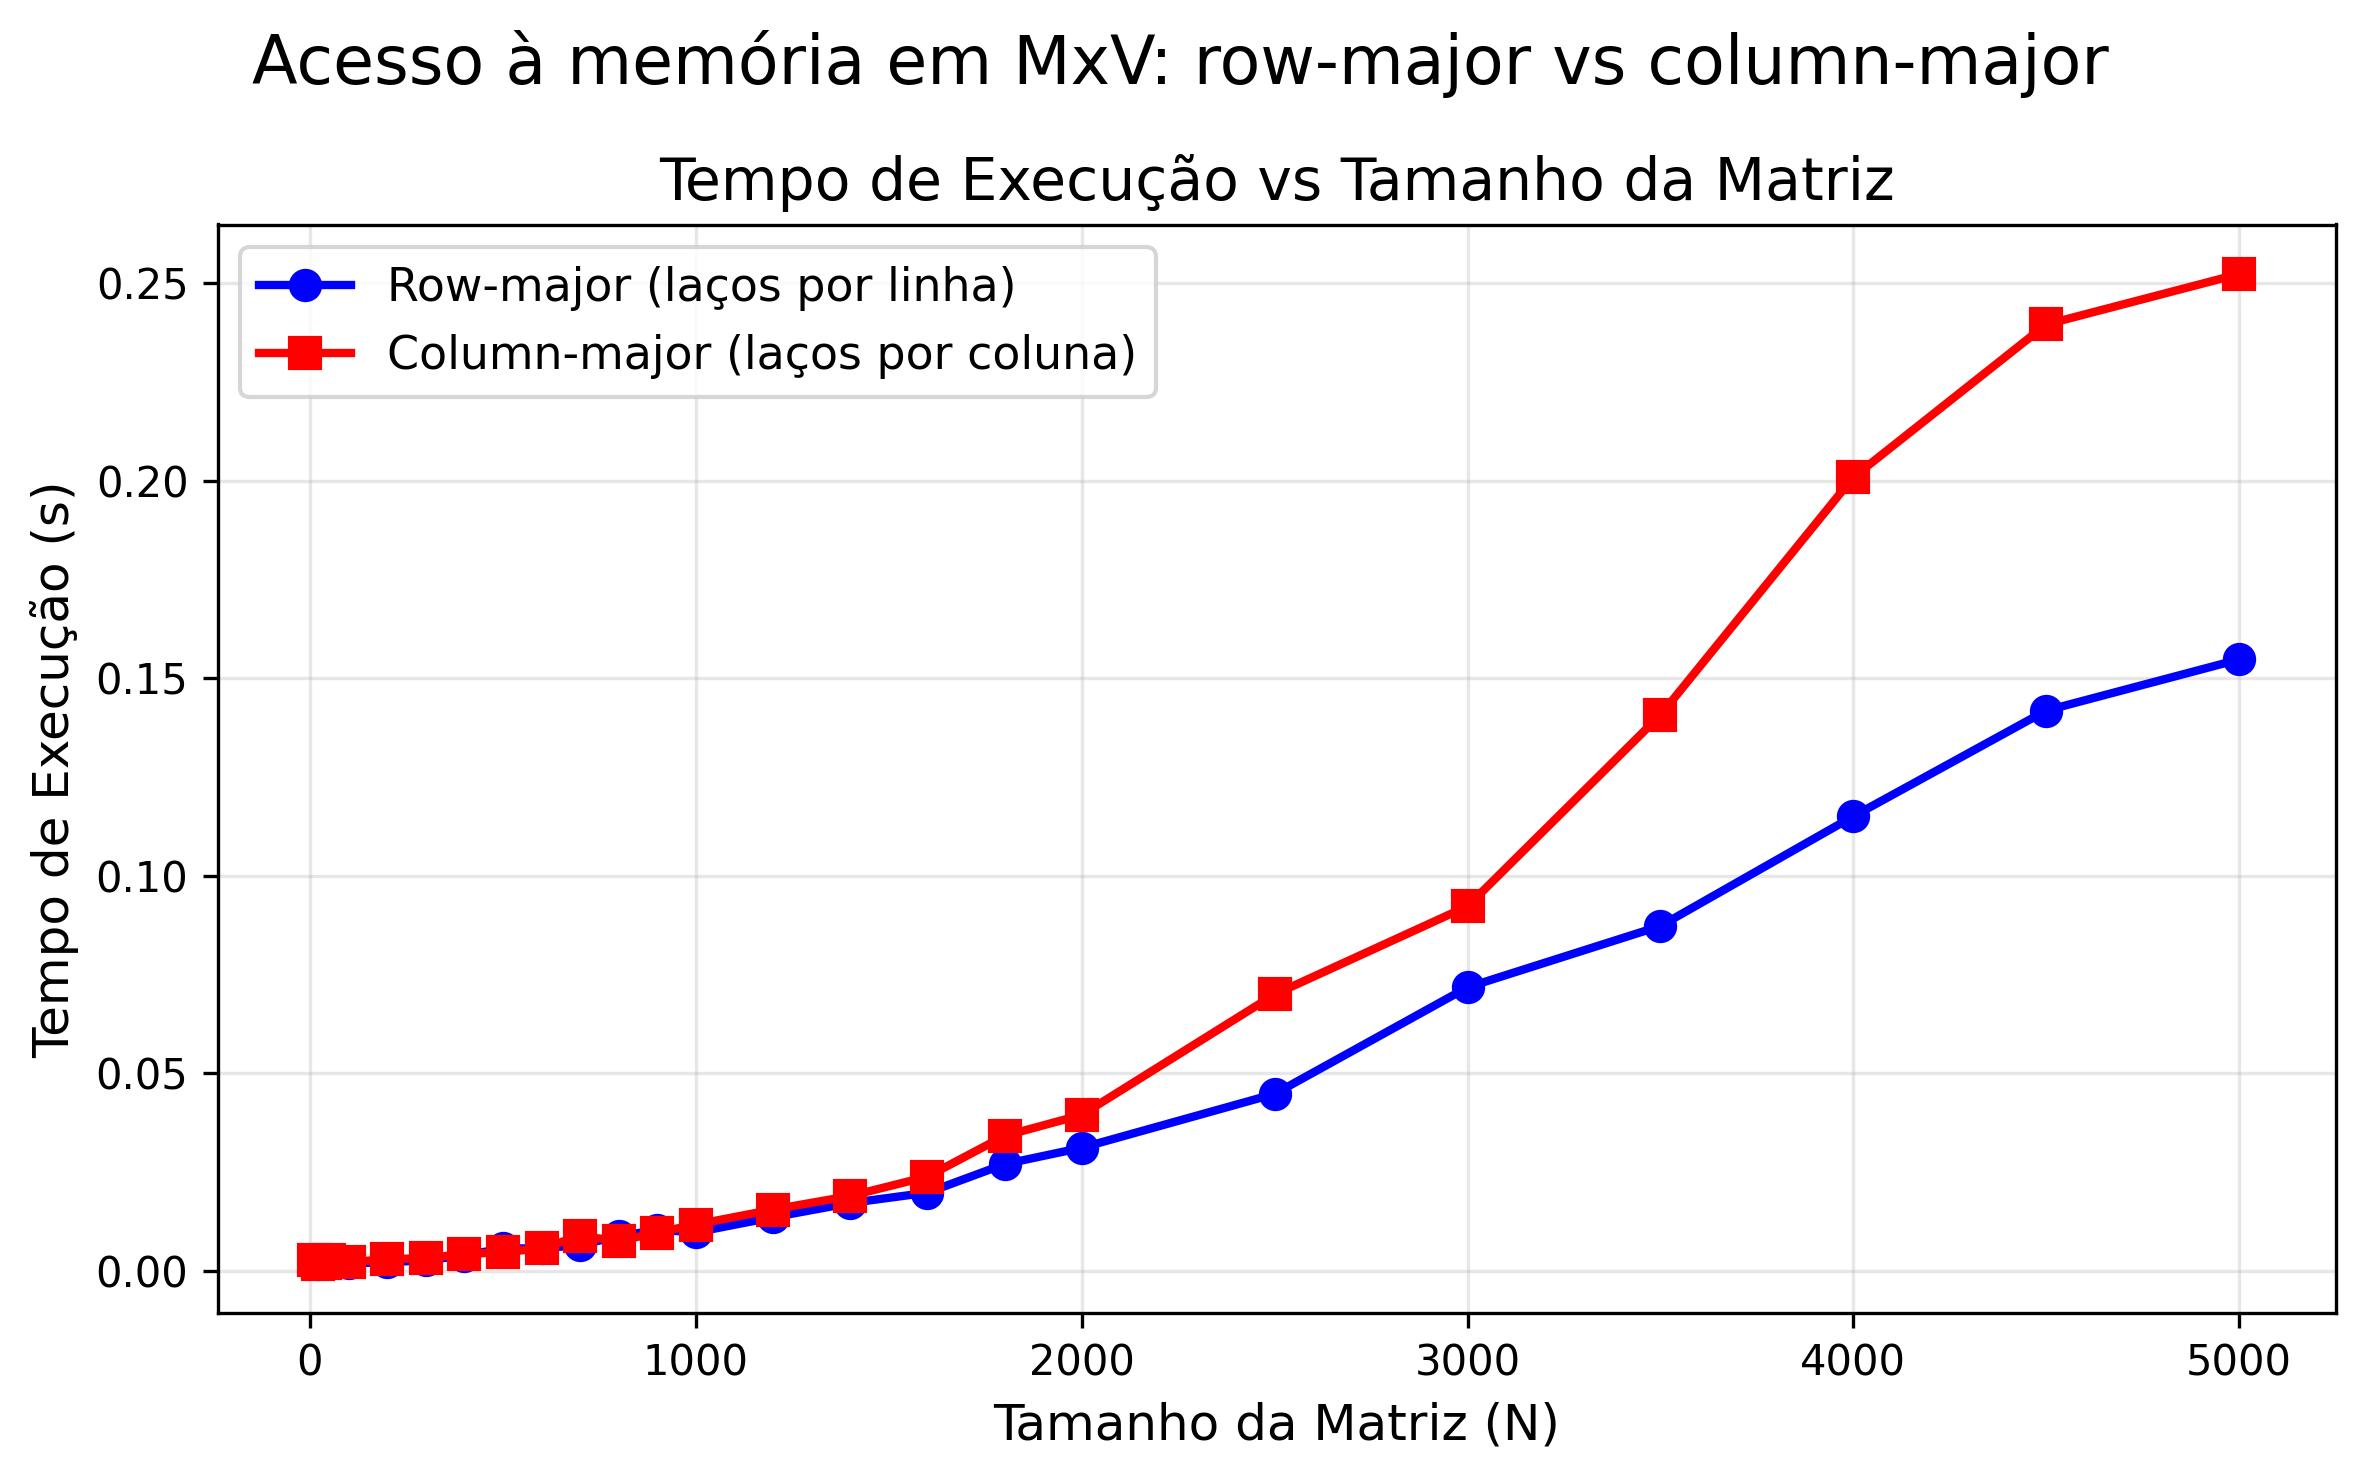
\includegraphics[width=0.9\textwidth]{mxv_memory_analysis.png}
\caption{Tempo de execução em função do tamanho da matriz $N$. A divergência entre as versões acentua-se nos maiores tamanhos.}
\label{fig:analysis}
\end{figure}

Para matrizes pequenas ($N \le 600$), os dados cabem nos caches L1 e L2, e ambas as versões completam em menos de 6 milissegundos. A variabilidade da medição supera a diferença real entre os padrões de acesso nessa faixa.

A separação começa a se manifestar na faixa intermediária ($700 \le N \le 1600$), embora de forma não monotônica: em $N=500$, $N=800$ e $N=900$ a versão por colunas foi ligeiramente mais rápida, o que indica ruído experimental em medições de execução única. Esses casos não invalidam a tendência geral, mas reforçam a necessidade de repetições com mediana para isolar o sinal do ruído. Em $N=1600$, com a matriz ocupando 20,48 MB e excedendo o cache L2 de 2 MiB, a versão por colunas levou 20,6\% a mais (0,023868 s contra 0,019798 s).

Para matrizes grandes ($N \ge 2000$), a divergência consolida-se. Em $N=2500$ a matriz consome 50 MB ($8 \times 2500^2$ bytes), superando os 33 MiB do cache L3 compartilhado. As faltas de cache forçam buscas diretas na memória DRAM. Em $N=5000$ (matriz de 200 MB), a versão por colunas levou 0,252379 s contra 0,154810 s da versão por linhas, um acréscimo de 63,0\% no tempo total.

\newpage
\section{Discussão}

A divergência decorre da perda de localidade espacial no acesso por colunas. Quando o laço interno varia a linha $i$ com coluna $j$ constante, iterações consecutivas leem $A[i \cdot N + j]$ e $A[(i+1) \cdot N + j]$. A distância entre dois acessos sucessivos na memória é dada por:
\[
\text{Stride} = N \times \text{sizeof(double)} = 8N \text{ bytes}
\]

Para $N=2000$, o salto entre iterações é de 16.000 bytes, equivalente a um deslocamento de 250 linhas de cache ($16.000 / 64$). Cada iteração consome apenas 8 bytes e descarta os outros 56 bytes trazidos pela linha de cache.

Enquanto a matriz cabe nos caches L1 (até $N \approx 78$) e L2 (até $N \approx 512$), a penalidade por falta de cache é baixa (4 a 14 ciclos de clock). Conforme o volume de dados excede o cache L2 e satura o cache L3 (33 MiB, superado em $N \approx 2080$), as faltas de cache recorrentes transferem a carga para a DRAM, cuja latência alcança 150 a 200 ciclos. O mecanismo de \textit{hardware prefetcher} do processador também perde eficácia com passos de memória tão amplos, incapaz de antecipar o fluxo de dados não-contíguo.

\section{Conclusão}

O experimento mostra que a ordem dos laços na multiplicação matriz-vetor determina o desempenho em arquiteturas modernas. Para matrizes pequenas ($N \le 600$), os dados cabem nos caches L1 e L2, mantendo os tempos de ambas as abordagens equivalentes.

A divergência estabiliza-se a partir de $N \approx 1600$ e amplia-se quando o volume de dados supera os 33 MiB do cache L3 ($N \ge 2500$). Em $N=5000$, o acesso por colunas leva 0,252 s contra 0,155 s do acesso por linhas, uma penalidade de 63,0\% decorrente do desperdício de 87,5\% de cada linha de cache e da sobrecarga na memória principal. Em C e em ambientes com armazenamento \textit{row-major}, alinhar a iteração dos laços à disposição contígua da memória é necessário para o aproveitamento da hierarquia de cache.

\end{document}